\begin{center}	
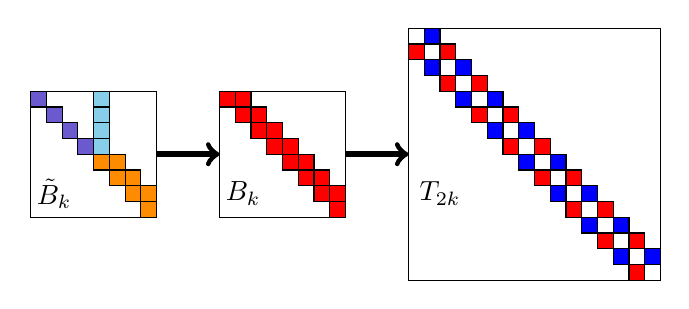
\begin{tikzpicture}[scale=.4]
  \pgfmathsetmacro{\ix}{1}

  \pgfmathsetmacro{\ix}{.5}
  \begin{scope}[shift={(0:4)}]
    \draw[fill=white] (0,-2) rectangle +(4,4);
    \foreach \x in { 0,...,3 }
    \draw[fill=SlateBlue] (\x*\ix,2-\ix-\x*\ix) rectangle +(\ix,\ix);
    \foreach \x in { 0,...,3 }
    \draw[fill=SkyBlue] (2,\x*\ix) rectangle +(\ix,\ix);
    \foreach \x in { 4,...,7 }
    \draw[fill=DarkOrange] (\x*\ix,2-\ix-\x*\ix) rectangle +(\ix,\ix);
    \foreach \x in { 4,...,6 }
    \draw[fill=DarkOrange] (\x*\ix+\ix,2-\ix-\x*\ix) rectangle +(\ix,\ix);
    \draw (0.75,-1.25) node{$\tilde{B}_k$};
  \end{scope}

  \begin{scope}[shift={(0:8)}]
      \draw [->,thick,line width=2pt] (0,0) -- (2,0);
  \end{scope}

  \begin{scope}[shift={(0:10)}]
    \draw[fill=white] (0,-2) rectangle +(4,4);
    \foreach \x in { 0,...,7 }
    \draw[fill=red] (\x*\ix,2-\ix-\x*\ix) rectangle +(\ix,\ix);
    \foreach \x in { 0,...,6 }
    \draw[fill=red] (\x*\ix+\ix,2-\ix-\x*\ix) rectangle +(\ix,\ix);
    \draw (0.75,-1.25) node{$B_k$};
  \end{scope}

  \begin{scope}[shift={(0:14)}]
      \draw [->,thick,line width=2pt] (0,0) -- (2,0);
  \end{scope}

  \begin{scope}[shift={(0:16)}]
    \draw[fill=white] (0,-4) rectangle +(8,8);
    \foreach \x in { 0,2,...,14 }
    \draw[fill=blue] (\x*\ix+\ix,4-\ix-\x*\ix) rectangle +(\ix,\ix);
    \foreach \x in { 1,3,...,13 }
    \draw[fill=blue] (\x*\ix,3-\x*\ix) rectangle +(\ix,\ix);
    \foreach \x in { 1,3,...,13 }
    \draw[fill=red] (\x*\ix+\ix,4-\ix-\x*\ix) rectangle +(\ix,\ix);
    \foreach \x in { 0,2,...,14 }
    \draw[fill=red] (\x*\ix,3-\x*\ix) rectangle +(\ix,\ix);
    \draw (1,-1.25) node{$T_{2k}$};
  \end{scope}
\end{tikzpicture}
\end{center}

